\documentclass[a4paper,11pt]{amsart}

\usepackage{gensymb}

\usepackage{tikz}
\usetikzlibrary{arrows.meta}
\usepackage{caption}

\usepackage{times}
\usepackage[top=27mm, left=23mm, bottom=23mm, right=23mm]{geometry}
\usepackage{amsfonts, amssymb, amsgen, amsthm, amscd, amsmath}
\usepackage{mathtools}
\mathtoolsset{showonlyrefs=true}

\usepackage{bm}
%\usepackage{mathpazo}
\usepackage{domitian}
\usepackage[T1]{fontenc}
\let\oldstylenums\oldstyle

\usepackage{enumerate}
\usepackage{color}
\usepackage[all]{xy}

\newtheorem{theorem}{Theorem}[section]
\newtheorem{proposition}[theorem]{Proposition}
\newtheorem{lemma}[theorem]{Lemma}
\newtheorem{corollary}[theorem]{Corollary}
\newtheorem{claim}[theorem]{Claim}
\theoremstyle{definition}
\newtheorem{remark}[theorem]{Remark}
\newtheorem{example}[theorem]{Example}
\newtheorem{definition}[theorem]{Definition}

\newcommand{\outimes}[2]{\overset{#1}{\underset{#2}{\otimes}}}
\newcommand{\C}[1]{\mathcal{#1}}
\newcommand{\B}[1]{\mathbb{#1}}
\newcommand{\G}[1]{\mathfrak{#1}}
\newcommand{\rmod}[1]{\text{{\bf Mod}-}{#1}}

\newcommand{\Span}{\text{\rm Span}}
\newcommand{\Tor}{\text{\rm Tor}}
\newcommand{\Ind}{\text{\rm Ind}}
\newcommand{\Res}{\text{\rm Res}}
\newcommand{\Ext}{\text{\rm Ext}}
\newcommand{\Hom}{\text{\rm Hom}}
\newcommand{\CoInd}{\text{\rm CoInd}}
\newcommand{\Simp}{{\Delta}}
\newcommand{\Diff}{{\Omega}}
\newcommand{\xla}[1]{\xleftarrow{#1}}
\newcommand{\colim}{\text{colim}}
\renewcommand{\baselinestretch}{1.15}

\setlength{\parskip}{1.2mm}
\setlength{\parindent}{0mm}

\title{Electromagnetism Assignment For The Second Time}

\author{Haixuan Lin - 23307110267}
\email{23307110267@m.fudan.edu.cn}


\address{Fudan University, Physics Department, China}

\begin{document}
	
	\begin{abstract}
		Here is the electromagnetism assignment for the first time which is for the corse given by professor Weichao Liu. In order to practise the expertise in scientific film of physics, students need to practise using \LaTeX to composing their own work, even if this is only a ordinary homework.
	\end{abstract}
	
	\maketitle
	\section*{Main Text}
	\subsection*{1-16}
	Let the point charge $q$ on the central axis gets a potential $\varphi$ from the thin ring when the distance from the center of a thin ring with charge $Q$ is $z$:
	\begin{equation*}
		\varphi=\frac{1}{4\pi \varepsilon _0}\frac{Q}{\sqrt{a^2+z^2}}
	\end{equation*}
	That because every tiny electronic part of thin ring has the same form of potential so the result is like above.
	The potential is a scalar quantity, according to the superposition principle:
	\begin{align*}
		\varPhi _1&=\frac{1}{4\pi \varepsilon _0}\left( \frac{q_1}{a}+\frac{q_2}{\sqrt{a^2+b^2}} \right)=\frac{A_1}{q}
		\\
		\varPhi _2&=\frac{1}{4\pi \varepsilon _0}\left( \frac{q_1}{\sqrt{a^2+b^2}}+\frac{q_2}{a} \right) =\frac{A_2}{q}
	\end{align*}
	So:
	\begin{align*}
		q_1&=\frac{4\pi \varepsilon _0}{b^2q}a\sqrt{a^2+b^2}\left( \sqrt{a^2+b^2}A_1-aA_2 \right) 
		\\
		q_1&=\frac{4\pi \varepsilon _0}{b^2q}a\sqrt{a^2+b^2}\left( \sqrt{a^2+b^2}A_2-aA_1 \right) 
	\end{align*}
	
	

	\begin{minipage}{0.5\textwidth}
		\subsection*{1-19}
		\subsubsection*{(1)}
		According to the assumption, the potential gradient between the grid is uniform, that is, the potential varies linearly with distance, and the cathode is the zero point of the potential.
	\end{minipage}
	\begin{minipage}{0.5\textwidth}
		\centering
		\begin{tikzpicture}
			\draw[->] (0, 0) -- (5, 0) node[right] {$x$};
			\draw[->] (0, -0.5) -- (0, 3.5) node[above] {$U$};
			\draw[thick] (0, 0) -- (1, 3) -- (5, 2.5);
		\end{tikzpicture}
	\end{minipage}
	\subsubsection*{(2)}
	According to classical mechanics, the kinetic energy theorem is listed.
	\begin{equation*}
		eU_+=\frac{1}{2}m_{\mathrm{e}}v^2
	\end{equation*}
	So $\displaystyle v=\sqrt{\dfrac{2eU_+}{m_\mathrm{e}}}\approx 2.30\times10^6\thinspace m/s.$
	
	\subsection*{1-20}
	It's easy to draw the electric field given by each plate.
	
	\begin{figure}[htbp]
		\begin{minipage}{0.49\textwidth}
			\centering
			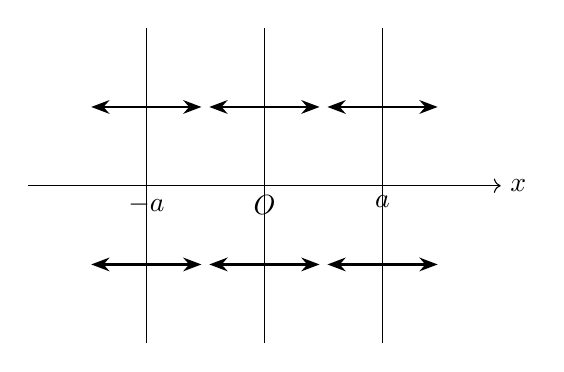
\begin{tikzpicture}
				\draw[->] (-3, 0) -- (-1.5, 0) node[below] {$-a$} -- (0, 0) node[below] {$O$} -- (1.5, 0) node[below] {$a$} -- (3, 0) node[right] {$x$};
				\draw (-1.5, -2) -- (-1.5, 2) (0, -2) -- (0, 2) (1.5, -2) -- (1.5, 2);
				\draw[-Stealth, thick] (-1.5, 1) -- (-0.8, 1);
				\draw[-Stealth, thick] (-1.5, 1) -- (-2.2, 1);
				\draw[-Stealth, thick] (-1.5, -1) -- (-0.8, -1);
				\draw[-Stealth, thick] (-1.5, -1) -- (-2.2, -1);
				\draw[-Stealth, thick] (0, 1) -- (-0.7, 1);
				\draw[-Stealth, thick] (0, 1) -- (0.7, 1);
				\draw[-Stealth, thick] (0, -1) -- (-0.7, -1);
				\draw[-Stealth, thick] (0, -1) -- (0.7, -1);
				\draw[-Stealth, thick] (1.5, 1) -- (0.8, 1);
				\draw[-Stealth, thick] (1.5, 1) -- (2.2, 1);
				\draw[-Stealth, thick] (1.5, -1) -- (0.8, -1);
				\draw[-Stealth, thick] (1.5, -1) -- (2.2, -1);
			\end{tikzpicture}
			\captionof*{figure}{Befor each electric field \\ is superimposed} % 需要 caption 宏包
			% 或者如果不想用 caption 宏包:
			%\textbf{BE}
		\end{minipage}
		\begin{minipage}{0.49\textwidth}
			\centering
			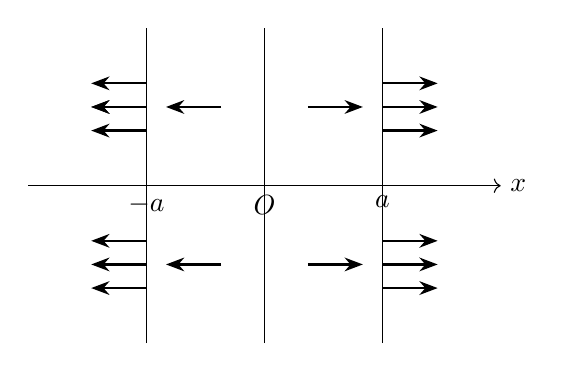
\begin{tikzpicture}
				\draw[->] (-3, 0) -- (-1.5, 0) node[below] {$-a$} -- (0, 0) node[below] {$O$} -- (1.5, 0) node[below] {$a$} -- (3, 0) node[right] {$x$};
				\draw (-1.5, -2) -- (-1.5, 2) (0, -2) -- (0, 2) (1.5, -2) -- (1.5, 2);
				%\draw[-Stealth, thick] (-1.5, 1) -- (-0.8, 1);
				\draw[-Stealth, thick] (-1.5, 1) -- (-2.2, 1);
				%\draw[-Stealth, thick] (-1.5, -1) -- (-0.8, -1);
				\draw[-Stealth, thick] (-1.5, 1) -- (-2.2, 1);
				\draw[-Stealth, thick] (-1.5, -1) -- (-2.2, -1);
				%\draw[-Stealth, thick] (0, 1) -- (-0.7, 1);
				%\draw[-Stealth, thick] (0, 1) -- (0.7, 1);
				%\draw[-Stealth, thick] (0, -1) -- (-0.7, -1);
				%\draw[-Stealth, thick] (0, -1) -- (0.7, -1);
				%\draw[-Stealth, thick] (1.5, 1) -- (0.8, 1);
				\draw[-Stealth, thick] (1.5, 1) -- (2.2, 1);
				%\draw[-Stealth, thick] (1.5, -1) -- (0.8, -1);
				\draw[-Stealth, thick] (1.5, -1) -- (2.2, -1);
				
				\draw[-Stealth, thick] (-1.5, 1.3) -- (-2.2, 1.3);
				\draw[-Stealth, thick] (-1.5, -1.3) -- (-2.2, -1.3);
				\draw[-Stealth, thick] (-1.5, 0.7) -- (-2.2, 0.7);
				\draw[-Stealth, thick] (-1.5, -0.7) -- (-2.2, -0.7);
				
				\draw[-Stealth, thick] (1.5, 1.3) -- (2.2, 1.3);
				\draw[-Stealth, thick] (1.5, -1.3) -- (2.2, -1.3);
				\draw[-Stealth, thick] (1.5, 0.7) -- (2.2, 0.7);
				\draw[-Stealth, thick] (1.5, -0.7) -- (2.2, -0.7);
				
				\draw[-Stealth, thick] (-0.55, 1) -- (-1.25, 1);
				\draw[-Stealth, thick] (-0.55, -1) -- (-1.25, -1);
				
				\draw[-Stealth, thick] (0.55, 1) -- (1.25, 1);
				\draw[-Stealth, thick] (0.55, -1) -- (1.25, -1);
			\end{tikzpicture}
			\captionof*{figure}{After each electric field \\ is superimposed} % 需要 caption 宏包
			% 或者如果不想用 caption 宏包:
			%\textbf{BE}
		\end{minipage}
	\end{figure}
	Where each face gives its half of the electric field strength is
	\begin{equation}
		E_0=\dfrac{\sigma}{2\varepsilon_0}
	\end{equation}
	So
	$$
	E(x)=\left\{
		\begin{aligned}
			-&\frac{3\sigma}{2\varepsilon _0}\qquad x<-a\\
			-&\frac{\sigma}{2\varepsilon _0}\qquad -a<x<0\\
			&\frac{\sigma}{2\varepsilon _0}\qquad 0<x<a\\
			&\frac{3\sigma}{2\varepsilon _0}\qquad a<x\\
		\end{aligned}
	\right.
	$$
	Integrate this function immediately:
	$$
	\varphi(x)=\left\{
	\begin{aligned}
		-&\frac{\sigma}{2\varepsilon _0}\left( a+3x \right) \qquad x<-a\\
		-&\frac{\sigma}{2\varepsilon _0}x\qquad -a<x<0\\
		&\frac{\sigma}{2\varepsilon _0}x\qquad 0<x<a\\
		&\frac{\sigma}{2\varepsilon _0}\left( a+3x \right)\qquad a<x\\
	\end{aligned}
	\right.
	$$


	\subsection*{1-21}
	First prove that the electric field on the plane has no horizontal component:
	
	Assuming that there is a horizontal component, then the negative half axis of $z$ is supplemented with half a spherical shell to form a complete spherical shell, then according to the symmetry, the lower half of the spherical shell also contributes the same horizontal electric field, then the interior of the entire spherical shell has a horizontal electric field in the $Oxy$ plane, which is contradictory to the conclusion that there is no electric field inside the uniform charged spherical shell.
	
	So the potential is equal everywhere in the $Oxy$ plane of the hemispherical shell, we just need to find the potential at $O$.
	
	The potential contribution of any element on the shell is the same, so
	\begin{equation*}
		\varphi =\frac{1}{4\pi \varepsilon _0}\frac{2\pi R^2\sigma}{R}=\frac{R\sigma}{2\varepsilon _0}
	\end{equation*}
	
	\subsection*{1-23}
	\subsubsection*{(1)}
	It is obviously the same as the circular electric flux formed by the intersection line between the hemispherical surface and the Oxy plane.
	$$
	\varPhi _{\mathrm{E}}=\pi R^2E
	$$
	\subsubsection*{(2)}
	In other words, the normal of the circle will be at an Angle of $60\degree$ to the strength of the electric field.
	$$
	\varPhi _{\mathrm{E}}^{'}=\varPhi _{\mathrm{E}}\cos 60\degree=\frac{1}{2}\pi R^2E
	$$
	\bibliographystyle{siam}
	\bibliography{C:/Users/Administrator/Desktop/VScode/LaTeX/arXiv-2402.19291v1/main.bbl}
	
	\subsection*{1-26}
	\subsubsection*{(1)}
	Consider the energy.
	$$
	\frac{1}{2\pi\varepsilon_0}\frac{Q_\alpha Q_\mathrm{Au}}{r_\mathrm{min}}=\frac{1}{2}m_\alpha v_0^2
	$$
	So $\displaystyle r_\mathrm{min}=\frac{1}{2\pi \varepsilon _0}\frac{Q_{\alpha}Q_{\mathrm{Au}}}{m_{\alpha}v_{0}^{2}}\approx4.25\times10^{-14}\thinspace\mathrm{m}.$
	\subsubsection*{(2)}
	Consider energy in two phases.
	$$
	(E_\mathrm{k})_\mathrm{min}=\frac{1}{4\pi \varepsilon _0}\frac{Q_{\alpha}Q_{\mathrm{Au}}}{r_{\mathrm{Au}}}+\int_0^{r_{\mathrm{Au}}}{E\left( r \right) \mathrm{d}r}
	$$
	According to Gauss theorem.
	$$
	4\pi r^2E\left( r \right) =\frac{r^3}{r_{\mathrm{Au}}^{3}}Q_{\mathrm{Au}}
	$$
	So $\displaystyle\left( E_{\mathrm{k}} \right) _{\min}=\frac{1.5}{4\pi \varepsilon _0}\frac{Q_{\alpha}Q_{\mathrm{Au}}}{r_{\mathrm{Au}}}\approx7.29\times10^{-12}\thinspace\mathrm{J}$.
	\subsection*{1-27}
	\subsubsection*{(1)}
	According to Gauss's theorem of free space:
	$$
	\nabla \cdot \boldsymbol{E}=\frac{\rho \left( r \right)}{\varepsilon _0}
	$$
	Where $\nabla$ is the Hamiltonian operator, in spherical coordinates, if the system is spherically symmetric, then
	$$
	\nabla =\frac{1}{r^2}\frac{\partial}{\partial r}r^2\hat{\boldsymbol{r}}
	$$
	Consider Electrons are negatively charged
	$$
	\frac{1}{r^2}\frac{\partial}{\partial r}r^2E\left( r \right) =-\frac{e}{\pi a_{0}^{3}}\mathrm{e}^{-\tfrac{2r}{a_0}}
	$$
	Because the system is spherically symmetric
	$$
	\frac{\partial}{\partial r}=\frac{\mathrm{d}}{\mathrm{d}r}
	$$
	Solving this equation above gives us
	$$
	r^2E\left( r \right) =\frac{e}{\pi\varepsilon_0}\left( \frac{1}{2a_{0}^{2}}r^2+\frac{1}{2a_0}r+\frac{1}{4} \right) \mathrm{e}^{-\tfrac{2r}{a_0}}
	$$
	That is
	$$
	E\left( r \right) =\frac{e}{\pi\varepsilon_0}\left( \frac{1}{4}\frac{1}{r^2}+\frac{1}{2a_0}\frac{1}{r}+\frac{1}{2a_{0}^{2}} \right) \mathrm{e}^{-\tfrac{2r}{a_0}}
	$$
	\subsubsection*{(2)}	
	Get by substitution
	$$
	E\left( a_0 \right) =\frac{5\mathrm{e}^{-2}e}{4\pi \varepsilon _0a_{0}^{2}}\approx3.47\times10^{11}\thinspace \mathrm{N/C}
	$$
	But
	$$
	E_{class}(a_0)=\frac{e^2}{4\pi \varepsilon _0a_{0}}\approx5.13\times10^{11}\thinspace \mathrm{N/C}
	$$
	So here is
	$$
	E_{class}(a_0)<E(a_0)
	$$
	\subsection*{1-31}
	Write down the potential energy of the electron
	$$
	U\left( r \right) =\frac{1}{4\pi \varepsilon _0}\frac{\tfrac{r^3}{R^3}Qe}{r}=\frac{1}{2}\frac{Qe}{2\pi \varepsilon _0R^3}r^2
	$$
	Compared with the energy of the spring oscillator, the equivalent recovery coefficient $\mathcal{K}$ is obtained.
	$$
	\mathcal{K} =\frac{Qe}{2\pi \varepsilon _0R^3}
	$$
	Apply the formula of simple harmonic motion
	$$
	f=\dfrac{1}{T}=\dfrac{1}{2\pi}\sqrt{\dfrac{\mathcal{K}}{m}}=\frac{1}{2\pi}\sqrt{\frac{Qe}{2\pi \varepsilon _0R^3m}}
	$$
\end{document}

